\chapter{Main Board}
\section{Introduction}
For our project we need a common power supply and connection platform for all the robot parts. This board should provide different levels of power supply for different purposes (drives, sensor, FPGA) and space  to connect all necessary hardware.

We chose 20 V 3 A as our input power supply. 

\section{Components choice and design implementation}

 For the 12 V power supply we chose linear regulator TS7812 \cite{linear_regulator}, with the recommended set up. The linear regulators are low in effieciency, but are easy to implement and have higher ripple rejection rates. The TS7812 is able to support up to 2 A of supply current which is sufficient for the motors We added 0.3 $\mu F$ an input $C_{in}$ and 0.1  $\mu F$ an output $C_{out}$ capacitor, following the data sheet. This regulator embeds internal current limiting, thermal shut-down and safe area protection, making it essentially indestructible.

\begin{figure}[!ht]
	\centering
	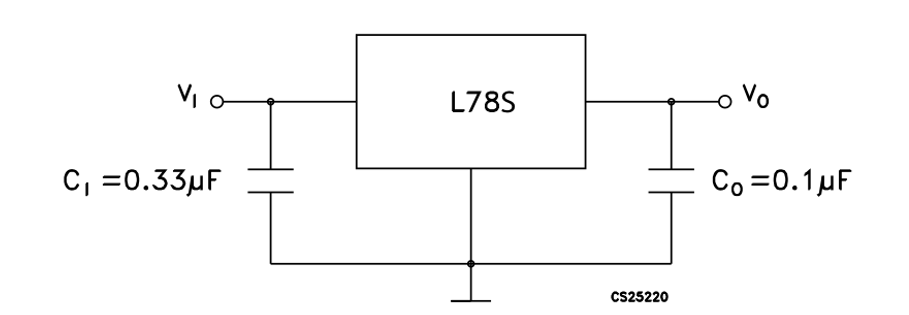
\includegraphics[width=1.0\textwidth]{figures/linear_regulator}
	\caption{TS7812 regulator implementation}
	\label{fig:linear_reg}
\end{figure}
 
  In the previous project we achieved on our main board around 11.96 V stable DC voltage. In this project we are using the 12 V input only to drive the motors. The maximum $V_{cc}$ for them is 12 V, so we wanted to achieve values around 12 V. With the current main board with the TS7812 linear regulator we get stable 11.70 V without any ripple (by the support from the used capacitors). This value could be raised for full 12 V by adding an additional circuit, but our purpose is to drive the motor with some reserve below 12 V so this 0.3 V difference is acceptable for us as the motors don't need to be run on maximum voltage. If we want to get full 12 V we simply change the new lighter and smaller main board for the old one that is able to supply with higher voltage. The boards are compatible. 
 
Besides the power supply for the motors we need power supply for other components (ADC, distance sensor) and the FPGA. We decided to implement a 5 V switching regulator with $LM2675N-ADJ Switching Regulator$ \cite{switching_regulator}. We chose this component because we had achieved very good results using it in previous project. The switching regulators are a bit more difficult to implement, but are more efficient than the linear regulators. According to the data sheet, its efficiency reaches up to 96 \%. The data sheet also guarantees 1 A output load current, which is enough to cover the need of all the specific circuits. 

\begin{figure}[!ht]
	\centering
	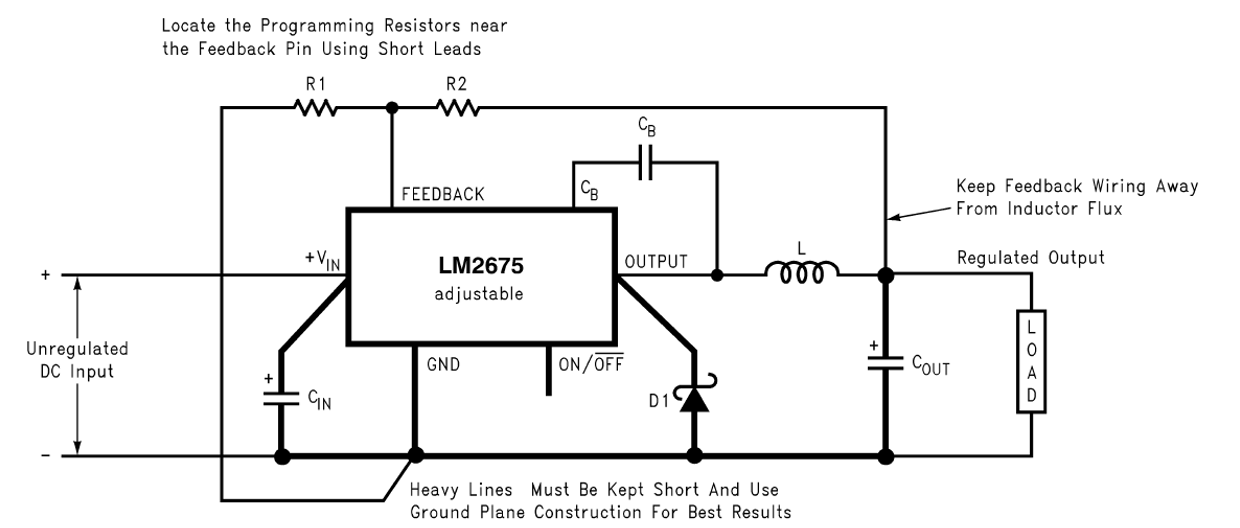
\includegraphics[width=1.0\textwidth]{figures/switching_regulator}
	\caption{Switching regulator implementation}
	\label{fig:linear_reg}
\end{figure}

The final PCB contains both power supply lines and interface to connect other PCBs. We have added several connectors for the FPGA, sensor board, H-bridge drive board, and also uTosNet connection. The board was design carefully designed to save more space. 
 
\section{Conclusions}
We have successfully designed a new light-weigh version of the main board more suitable for mounting on the robot chasis. This board is capable of power supplying the motors and also the FPGA, sensor and ADC (5 V). It provides an interface to connect different PCBs and also the uTosNet connection. 